\documentclass[11pt]{article}
\usepackage[a4paper,margin=2cm]{geometry}
\usepackage[T1]{fontenc}
\usepackage{lmodern,microtype}
\usepackage{amsmath,booktabs}
\usepackage[authoryear,round]{natbib}
\usepackage[hidelinks]{hyperref}
\usepackage{pgfplots}
\usepgfplotslibrary{groupplots,fillbetween}
\pgfplotsset{compat=1.18}
\usetikzlibrary{shapes.geometric}
\usepackage{caption}
\captionsetup{font=small,labelfont=bf}
\setlength{\textfloatsep}{12pt plus 2pt minus 4pt}
\setlength{\intextsep}{6pt plus 2pt minus 2pt}
\bibpunct{(}{)}{;}{a}{,}{,}

% Colours: TCGA-UT blue, BRACS orange.
\definecolor{cP}{HTML}{4575B4}
\definecolor{cS}{HTML}{91BFDB}
\definecolor{cI}{HTML}{FDAE61}
\definecolor{tcga}{HTML}{2166AC}
\definecolor{bracs}{HTML}{D6604D}

% Realized training class counts, sorted head to tail (exp-02 allocator; N = native shares of split 0, draw 0).
\pgfplotstableread{
rank r1 r2 r5 r10 r20 r50 r100 N
1 640 886 1278 1615 1973 2466 2843 1746
2 640 865 1209 1491 1780 2155 2426 1684
3 640 845 1144 1378 1605 1883 2070 1675
4 640 825 1082 1272 1448 1645 1766 1206
5 640 805 1024 1175 1305 1438 1506 1182
6 640 786 969 1086 1177 1256 1285 897
7 640 768 916 1003 1062 1098 1097 894
8 640 750 867 926 958 959 936 841
9 640 732 820 856 864 838 798 836
10 640 715 776 790 779 732 681 807
11 640 698 734 730 702 640 581 708
12 640 681 694 674 634 559 496 703
13 640 665 657 623 571 489 423 702
14 640 649 621 575 515 427 361 665
15 640 634 588 531 465 373 308 605
16 640 619 556 491 419 326 263 596
17 640 604 526 453 378 285 224 472
18 640 590 498 419 341 249 191 445
19 640 576 471 387 307 217 163 422
20 640 563 445 357 277 190 139 337
21 640 549 421 330 250 166 119 290
22 640 536 399 305 226 145 101 247
23 640 524 377 281 203 127 86 234
24 640 511 357 260 183 111 74 179
25 640 499 338 240 165 97 63 176
26 640 487 319 222 149 85 54 161
27 640 476 302 205 135 74 46 145
28 640 465 286 189 121 65 39 130
29 640 454 270 175 109 56 33 119
30 640 443 256 161 99 49 28 96
}\tcgacounts
\pgfplotstableread{
rank r1 r2 r5 r10 r20 r50 r100 N
1 320 441 622 766 908 1084 1206 678
2 320 392 476 522 551 565 560 556
3 320 350 364 356 335 294 260 459
4 320 312 278 242 203 153 120 176
5 320 278 213 165 123 80 56 129
6 320 247 163 112 75 42 26 127
7 320 220 124 77 45 22 12 115
}\bracscounts

\newcommand{\countlines}[1]{%
  \addplot[black,thick,mark=*,mark size=1pt] table[x=rank,y=r1]{#1};
  \addplot[red!80!black,thick,dashed,mark=square*,mark size=1pt] table[x=rank,y=N]{#1};
  \addplot[tcga,thick,mark=triangle*,mark size=1.4pt] table[x=rank,y=r100]{#1};}

\title{\vspace{-1cm}\LARGE Class Imbalance in Histopathology\vspace{-0.5em}}
\author{Yannik Queisler}
\date{September 25, 2026}

\begin{document}
\maketitle

\section{Motivation}
Histopathology datasets are long-tailed almost by construction. Common cancers and benign tissue dominate archives, while rare subtypes and atypical lesions, often the diagnostically decisive ones, contribute few patients and patches. BRACS, for example, was released with explicitly unbalanced atypical classes \citep{brancati2022bracs}. In CNNs, imbalance biases predictions toward frequent classes and lowers minority recall \citep{buda2018classImbalance}; in medical imaging it also distorts calibration, and conclusions depend on whether evaluation uses balanced metrics \citep{mosquera2024classImbalance}. Long-tailed medical benchmarks show that no single remedy works across datasets \citep{ju2024monicaBenchmark}, and histopathology-specific models keep being proposed \citep{cong2022imbalancedHistopathology}. Frozen foundation-model features with a linear probe are now the standard baseline \citep{chen2024uni,zimmermann2024virchow2}, yet how much imbalance still costs such a probe, and why, has not been sufficiently measured in isolation.

\section{Setup}
A multinomial logistic regression is trained on frozen Virchow2 patch features \citep{zimmermann2024virchow2} on two tasks: TCGA-UT, 30 cancer types \citep{komura2022universalEncoding}, and BRACS, 7 breast-lesion subtypes from normal tissue to invasive carcinoma \citep{brancati2022bracs}. Every condition uses the same patients per class (20 on TCGA-UT, 10 on BRACS) and the same total patch budget; only the share of that budget each class receives changes. An exponential profile sets the ratio $\rho$ between the largest and smallest class to 1--100 (Figure~\ref{fig:dist}), class-to-rank assignment is randomized over 30 draws (3 splits $\times$ 10), and a native condition keeps each dataset's own class shares. The outcome is the \emph{damage} $\Delta(\rho)=\mathrm{BA}(1)-\mathrm{BA}(\rho)$, the loss in test patient-macro balanced accuracy against the balanced condition, with paired bootstrap 95\% intervals; damage counts as material from 1 percentage point (pp).

\begin{figure}[!htb]
\centering
\begin{tikzpicture}
\begin{groupplot}[group style={group size=2 by 1,horizontal sep=1.3cm},
  width=0.5\textwidth,height=4.7cm,xlabel={Class rank (head $\to$ tail)},
  ymin=0,scaled y ticks=false,
  tick label style={font=\scriptsize},label style={font=\small},title style={font=\small},
  enlarge x limits=0.03]
\nextgroupplot[title={(a) TCGA-UT (30 classes, $T=19{,}200$)},ylabel={Training patches},xmin=1,xmax=30,
  legend style={font=\scriptsize,at={(0.98,0.97)},anchor=north east,draw=none,fill=none},
  legend cell align=left]
\countlines{\tcgacounts}
\legend{balanced ($\rho=1$),native ($\rho=18.1$),$\rho=100$}
\nextgroupplot[title={(b) BRACS (7 classes, $T=2{,}240$)},xmin=1,xmax=7,xtick={1,...,7},
  legend style={font=\scriptsize,at={(0.98,0.97)},anchor=north east,draw=none,fill=none},legend cell align=left]
\countlines{\bracscounts}
\legend{balanced ($\rho=1$),native ($\rho=6.7$),$\rho=100$}
\end{groupplot}
\end{tikzpicture}
\caption{Training class distributions, classes sorted from head to tail: the balanced condition, the native class shares of one split, and the most imbalanced ratio condition. The tested ratios are $\rho\in\{1,2,5,10,20,50,100\}$; the profiles for $\rho=2$ to 50 lie between the balanced and the $\rho=100$ profile. Which class sits at which rank is randomized per draw.}
\label{fig:dist}
\end{figure}

\section{Effects of class imbalance}
Balanced accuracy reaches 72.1\% on TCGA-UT and 39.6\% on BRACS. Published evaluations show the same broad gap: ROI-level linear probes score 60--68\% on TCGA-UT \citep{mahmoodlab2025uniRepo}, while slide-level linear probes score 34.8--48.1\% on BRACS \citep{vaidya2025threads}. TCGA-UT spans cancer types across organs, while BRACS separates breast lesions with similar morphology, such as ADH and DCIS \citep{brancati2022bracs}. These results make the gap plausible, though their training budgets and evaluation units differ. This study computes patient-macro recall from patch predictions.

Imbalance damage differs strongly between the two tasks (Figure~\ref{fig:damage}a). On TCGA-UT it is small and accelerating: 0.57 pp at $\rho=10$, the 1-pp threshold only at $\rho=20$, and 2.91 pp [2.48, 3.34] at $\rho=100$. On BRACS it starts immediately and grows steadily by about 1.15 pp per doubling of $\rho$: 1.15 pp already at $\rho=2$, 4.02 pp at $\rho=10$, and 7.65 pp [5.77, 9.78] at $\rho=100$, a fifth of the balanced level. Both native allocations lie on their curves (1.18 and 4.05 pp). The aggregate hides a large shift of recall from tail to head: at $\rho=100$, the TCGA-UT tail third loses 11.8 pp while the head gains 5.4 pp; on BRACS the two tail classes drop from 38.7\% to 7.3\% recall. The predicted probabilities suffer far more than accuracy (Figure~\ref{fig:damage}b). The expected calibration error (ECE), the average gap between the model's confidence and its accuracy, rises from 5.5 to 17.8 pp on TCGA-UT and from 12.3 to 35.7 pp on BRACS at $\rho=100$: the model becomes overconfident, but uniformly so. A global confidence correction that divides all logits by one scalar fitted on validation data (temperature scaling; \citealp{guo2017calibration}) removes 92--96\% of the increase.

\begin{figure}[t]
\centering
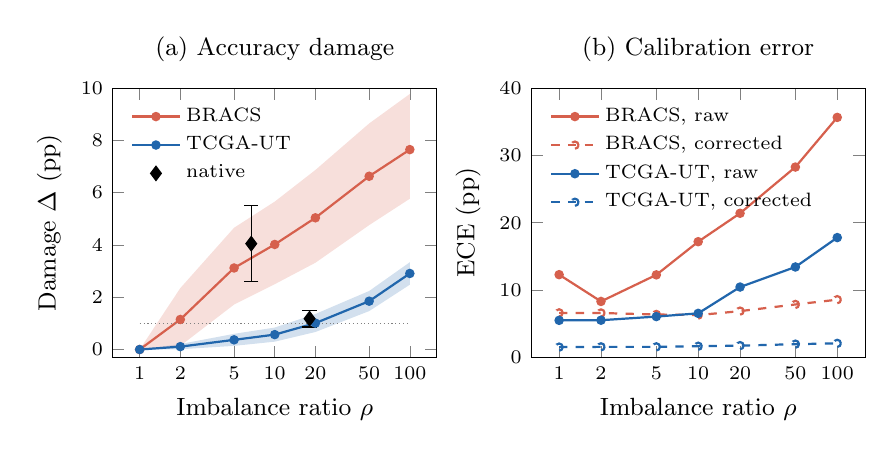
\begin{tikzpicture}
\begin{axis}[name=curve,title={(a) Accuracy damage},title style={font=\small},width=0.47\textwidth,height=5cm,xmode=log,log basis x=10,
  xtick={1,2,5,10,20,50,100},xticklabels={1,2,5,10,20,50,100},
  xlabel={Imbalance ratio $\rho$},ylabel={Damage $\Delta$ (pp)},ymin=-0.3,ymax=10,
  tick label style={font=\scriptsize},label style={font=\small},
  legend style={font=\scriptsize,at={(0.03,0.97)},anchor=north west,draw=none,fill=none},legend cell align=left]
\addplot[name path=tu,draw=none,forget plot] coordinates {(1,0)(2,0.21)(5,0.60)(10,0.84)(20,1.36)(50,2.24)(100,3.34)};
\addplot[name path=tl,draw=none,forget plot] coordinates {(1,0)(2,0.01)(5,0.14)(10,0.30)(20,0.67)(50,1.47)(100,2.48)};
\addplot[tcga,fill opacity=0.2,forget plot] fill between[of=tu and tl];
\addplot[name path=bu,draw=none,forget plot] coordinates {(1,0)(2,2.35)(5,4.66)(10,5.66)(20,6.87)(50,8.65)(100,9.78)};
\addplot[name path=bl,draw=none,forget plot] coordinates {(1,0)(2,0.14)(5,1.72)(10,2.50)(20,3.32)(50,4.76)(100,5.77)};
\addplot[bracs,fill opacity=0.2,forget plot] fill between[of=bu and bl];
\addplot[bracs,thick,mark=*,mark size=1.3pt] coordinates {(1,0)(2,1.15)(5,3.12)(10,4.02)(20,5.04)(50,6.63)(100,7.65)};
\addlegendentry{BRACS}
\addplot[tcga,thick,mark=*,mark size=1.3pt] coordinates {(1,0)(2,0.11)(5,0.37)(10,0.57)(20,1.01)(50,1.85)(100,2.91)};
\addlegendentry{TCGA-UT}
\addplot[only marks,mark=diamond*,mark size=2.6pt,black,error bars/.cd,y dir=both,y explicit]
  coordinates {(18.1,1.18) +- (0,0.32) (6.7,4.05) +- (0,1.45)};
\addlegendentry{native}
\draw[densely dotted,gray] (axis cs:1,1) -- (axis cs:100,1);
\end{axis}
\begin{axis}[at={(curve.east)},title={(b) Calibration error},title style={font=\small},anchor=west,xshift=1.2cm,width=0.48\textwidth,height=5cm,
  xmode=log,log basis x=10,xtick={1,2,5,10,20,50,100},xticklabels={1,2,5,10,20,50,100},
  xlabel={Imbalance ratio $\rho$},ylabel={ECE (pp)},ymin=0,ymax=40,
  tick label style={font=\scriptsize},label style={font=\small},
  legend style={font=\scriptsize,at={(0.03,0.97)},anchor=north west,draw=none,fill=none},legend cell align=left]
\addplot[bracs,thick,mark=*,mark size=1.3pt] coordinates {(1,12.29)(2,8.31)(5,12.26)(10,17.19)(20,21.41)(50,28.28)(100,35.66)};
\addlegendentry{BRACS, raw}
\addplot[bracs,thick,dashed,mark=o,mark size=1.3pt] coordinates {(1,6.61)(2,6.59)(5,6.37)(10,6.28)(20,6.87)(50,7.86)(100,8.57)};
\addlegendentry{BRACS, corrected}
\addplot[tcga,thick,mark=*,mark size=1.3pt] coordinates {(1,5.50)(2,5.52)(5,6.06)(10,6.54)(20,10.45)(50,13.43)(100,17.80)};
\addlegendentry{TCGA-UT, raw}
\addplot[tcga,thick,dashed,mark=o,mark size=1.3pt] coordinates {(1,1.52)(2,1.56)(5,1.56)(10,1.65)(20,1.74)(50,1.96)(100,2.08)};
\addlegendentry{TCGA-UT, corrected}
\end{axis}
\end{tikzpicture}
\caption{(a) Balanced-accuracy damage versus $\rho$ with 95\% bands; diamonds mark native class shares, dotted line the 1-pp threshold. (b) Expected calibration error (ECE) of the raw predicted probabilities (solid) and after a single global confidence correction fitted on validation data (dashed).}
\label{fig:damage}
\end{figure}

\section{Class influence and tail support}
\label{sec:cause}

When a tail class receives fewer training patches, two things change. Its errors count less often in the training loss, so common classes have more influence on the fitted decision boundary. This is the \emph{frequency} effect: it concerns how strongly the available examples of each class shape the classifier. The model also sees fewer distinct tail patches, at $\rho=100$ only one or two per patient, so it has less evidence about how that class varies. This is the \emph{support} effect: giving those few patches more weight cannot supply the missing examples. The conditions in Table~\ref{tab:conditions} separate these effects. F keeps all patches from the balanced condition but gives head classes more weight, isolating the frequency effect. S keeps the sparse patches from the imbalanced condition but weights classes equally, isolating the support effect. The interaction $I=\Delta_\mathrm{r}-\Delta_\mathrm{F}-\Delta_\mathrm{S}$ measures any additional damage when both occur together.

\begin{figure}[!htb]
\begin{minipage}[c]{0.48\textwidth}
\centering\small
\setlength{\tabcolsep}{3pt}
\begin{tabular}{@{}lcc@{}}
\toprule
Class influence & Many tail patches & Few tail patches \\
\midrule
Equal & balanced (ref.) & S: support only \\
Head-favoured & F: frequency only & r: ratio (both) \\
\bottomrule
\end{tabular}
\captionof{table}{Four training conditions separate the effect of unequal class influence (frequency) from the effect of fewer tail examples (support) at each $\rho$.}
\label{tab:conditions}
\end{minipage}\hfill
\begin{minipage}[c]{0.48\textwidth}
\centering
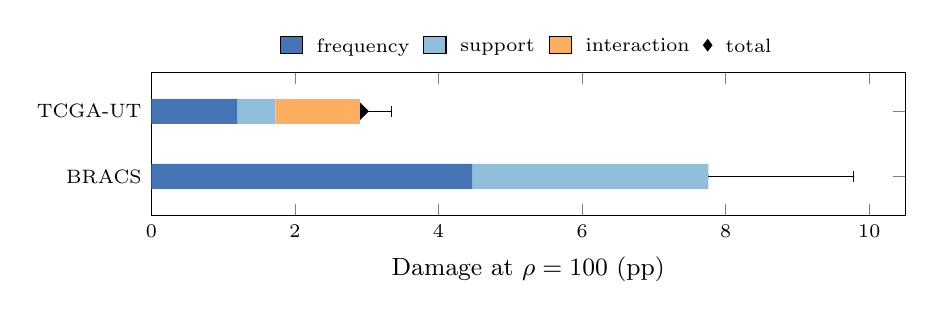
\begin{tikzpicture}
\begin{axis}[xbar stacked,width=0.92\linewidth,height=3.4cm,bar width=9pt,
  xmin=0,xmax=10.5,xlabel={Damage at $\rho=100$ (pp)},
  ytick={1,2},yticklabels={BRACS,TCGA-UT},ymin=0.4,ymax=2.6,
  tick label style={font=\scriptsize},label style={font=\small},
  legend style={font=\scriptsize,at={(0.5,1.03)},anchor=south,draw=none,fill=none,legend columns=4,column sep=3pt},
  legend cell align=left]
\addplot[fill=cP,draw=none] coordinates {(4.47,1) (1.20,2)};
\addlegendentry{frequency}
\addplot[fill=cS,draw=none] coordinates {(3.29,1) (0.53,2)};
\addlegendentry{support}
\addplot[fill=cI,draw=none] coordinates {(0,1) (1.18,2)};
\addlegendentry{interaction}
\addlegendimage{only marks,mark=diamond*,black}
\addlegendentry{total}
% Totals drawn outside the stack (an addplot here would stack onto the bars).
\draw[black,thin] (axis cs:5.77,1) -- (axis cs:9.78,1);
\draw[black,thin] ([yshift=-2pt]axis cs:5.77,1) -- ([yshift=2pt]axis cs:5.77,1);
\draw[black,thin] ([yshift=-2pt]axis cs:9.78,1) -- ([yshift=2pt]axis cs:9.78,1);
\node[diamond,fill=black,inner sep=1.6pt] at (axis cs:7.65,1) {};
\draw[black,thin] (axis cs:2.48,2) -- (axis cs:3.34,2);
\draw[black,thin] ([yshift=-2pt]axis cs:2.48,2) -- ([yshift=2pt]axis cs:2.48,2);
\draw[black,thin] ([yshift=-2pt]axis cs:3.34,2) -- ([yshift=2pt]axis cs:3.34,2);
\node[diamond,fill=black,inner sep=1.6pt] at (axis cs:2.91,2) {};
\end{axis}
\end{tikzpicture}
\caption{Damage at $\rho=100$ by component; diamonds give the total with its 95\% interval.}
\label{fig:decomp}
\end{minipage}
\end{figure}

\noindent The two tasks break down differently (Figure~\ref{fig:decomp}). On TCGA-UT the frequency effect carries the damage at moderate ratios (0.73 of 1.01 pp at $\rho=20$) while thin support alone costs nothing; at $\rho=100$ the two compound: frequency 1.20 pp [0.87, 1.53], support 0.53 pp [0.36, 0.70], and a clearly positive interaction of 1.18 pp [1.00, 1.37]. On BRACS both factors are material at $\rho=100$, frequency 4.47 pp [2.84, 6.30] and support 3.29 pp [1.99, 4.67], and their sum matches the total damage. The interaction is near zero, $-0.11$ pp, but its interval [$-1.74$, 1.36] cannot rule out compounding of up to 1.4 pp. Thin support alone thus costs BRACS more than the entire imbalance damage on TCGA-UT.

\section{Dependence on tail-class identity}

On BRACS, rotating every class through every rank shows that easy classes cost most when rare: damage at $\rho=100$ ranges from 5.73 pp (UDH in the tail) to 9.99 pp (invasive carcinoma), because a class with high balanced recall has the most to lose (Figure~\ref{fig:order}a). On TCGA-UT, a class is especially vulnerable when it receives few patches but a class it is often mistaken for receives many. A score fixed before testing new class orders used this pattern to predict their damage. The order ranked most damaging costs 4.51 pp, the least damaging 1.34 pp, and random orders 2.91 pp (Figure~\ref{fig:order}b). Reversing the most damaging order keeps the same rank gaps between pairs of classes but lowers damage by 1.11 pp [0.47, 1.73]. Damage is therefore greatest when the class prone to being mistaken for another is the rarer one.

\begin{figure}[!htb]
\centering
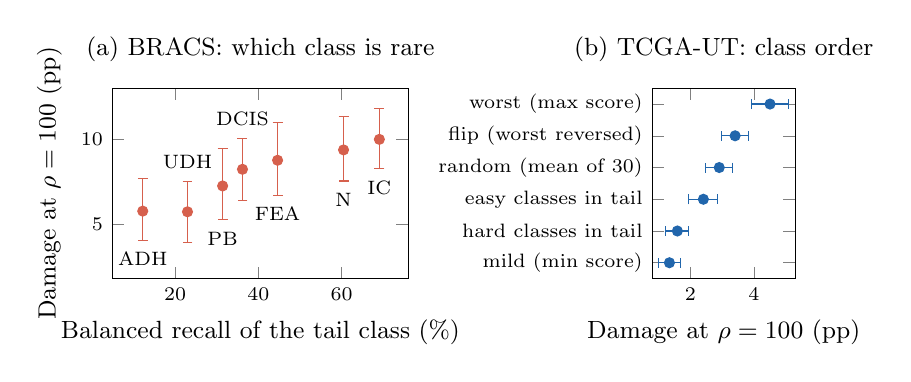
\begin{tikzpicture}
\begin{axis}[name=bracsorder,title={(a) BRACS: which class is rare},title style={font=\small},
  width=0.44\textwidth,height=4cm,xmin=5,xmax=76,ymin=1.8,ymax=13,clip=false,
  xlabel={Balanced recall of the tail class (\%)},ylabel={Damage at $\rho=100$ (pp)},
  tick label style={font=\scriptsize},label style={font=\small}]
\addplot[only marks,mark=*,bracs,mark size=1.8pt,error bars/.cd,y dir=both,y explicit]
  coordinates {(12.23,5.77) -= (0,1.71) += (0,1.92) (22.98,5.73) -= (0,1.80) += (0,1.79) (31.42,7.25) -= (0,1.99) += (0,2.19) (36.19,8.23) -= (0,1.81) += (0,1.82) (44.62,8.76) -= (0,2.05) += (0,2.24) (60.47,9.37) -= (0,1.83) += (0,1.95) (69.07,9.99) -= (0,1.73) += (0,1.81)};
\node[font=\scriptsize,below=1pt] at (axis cs:12.23,4.06) {ADH};
\node[font=\scriptsize,above=1pt] at (axis cs:22.98,7.52) {UDH};
\node[font=\scriptsize,below=1pt] at (axis cs:31.42,5.26) {PB};
\node[font=\scriptsize,above=1pt] at (axis cs:36.19,10.05) {DCIS};
\node[font=\scriptsize,below=1pt] at (axis cs:44.62,6.71) {FEA};
\node[font=\scriptsize,below=1pt] at (axis cs:60.47,7.54) {N};
\node[font=\scriptsize,below=1pt] at (axis cs:69.07,8.26) {IC};
\end{axis}
\begin{axis}[at={(bracsorder.east)},anchor=west,xshift=3.1cm,title={(b) TCGA-UT: class order},title style={font=\small},
  width=0.28\textwidth,height=4cm,xmin=0.8,xmax=5.3,ymin=0.5,ymax=6.5,
  ytick={1,...,6},yticklabels={mild (min score),hard classes in tail,easy classes in tail,random (mean of 30),flip (worst reversed),worst (max score)},
  xlabel={Damage at $\rho=100$ (pp)},tick label style={font=\scriptsize},label style={font=\small}]
\addplot[only marks,mark=*,tcga,mark size=1.8pt,error bars/.cd,x dir=both,x explicit]
  coordinates {(1.34,1) -= (0.34,0) += (0.35,0)
               (1.59,2) -= (0.37,0) += (0.36,0)
               (2.41,3) -= (0.46,0) += (0.44,0)
               (2.91,4) -= (0.43,0) += (0.43,0)
               (3.41,5) -= (0.43,0) += (0.43,0)
               (4.51,6) -= (0.58,0) += (0.57,0)};
\end{axis}
\end{tikzpicture}
\caption{Damage at $\rho=100$ with 95\% intervals. (a) BRACS with each class in the tail in turn, against its balanced-condition recall (Spearman 0.96, $n=7$). (b) TCGA-UT class-to-rank assignments.}
\label{fig:order}
\end{figure}

\section{Encoder comparison}
Refitting all conditions on identical patients with UNI2-h \citep{chen2024uni} instead of Virchow2 leaves the picture intact. On TCGA-UT, UNI2-h starts 1.78 pp higher and loses 0.86 pp less at $\rho=100$ (97.5\% interval 0.40 to 1.33), a resolved but sub-1-pp difference. On BRACS the difference is unresolved and the tail classes collapse to about 9\% recall with both encoders.

\section{Implications for mitigation}
\begin{itemize}\setlength{\itemsep}{1pt}
\item Rebalancing the training objective removes the frequency damage but cannot restore thin support. On BRACS, 3.3 pp remain at $\rho=100$; recovering them needs more tail patches or patients, or methods that improve tail-class estimation.
\item Confidence correction removes most calibration damage; mitigation must beat that baseline.
\item At the same $\rho$, damage varies 2--3-fold with dataset and class order; randomize class order.
\end{itemize}

\clearpage
\appendix
\section{Guide to the supporting experiments}
The numbered folders below are under \path{experiments/03_class_imbalance/}. Each folder's \path{report/} directory contains a PDF and its LaTeX source. The reports give the protocols, full tables, and uncertainty estimates behind the results condensed here.\\

\noindent\textbf{Headline results.}
\begin{itemize}\setlength{\itemsep}{2pt}
\item \textbf{Imbalance curves and probability quality:} Reports 25 and 26, in \path{00_damage/25_damage_tcga_ut/report/} and \path{00_damage/26_damage_bracs/report/}, give the balanced baselines, damage at every ratio, native allocations, head-to-tail recall, and calibration before and after temperature scaling.
\item \textbf{Class influence versus tail support:} Reports 27 and 28, in \path{01_cause/tcga_ut/27_prior_vs_support/report/} and \path{01_cause/bracs/28_prior_vs_support/report/}, show the paired frequency-only (called prior-only, P, in the reports) and support-only conditions, their interaction, and its uncertainty on each dataset.
\item \textbf{Which classes become rare:} Report 29, in \path{01_cause/bracs/29_tail_assignment/report/}, rotates every BRACS class through the tail. Report 32, in \path{01_cause/tcga_ut/32_worst_assignment_rate/report/}, tests predicted damaging and mild class orders on TCGA-UT, including reversal of the most damaging order.
\item \textbf{Encoder comparison:} Report 39, in \path{01_cause/cross/39_encoder_transfer/report/}, compares Virchow2 and UNI2-h on matched patients and patches and examines sensitivity to regularization selection.
\end{itemize}

\noindent\textbf{Further reading.} Reports 25 and 26 also track negative log-likelihood and fitted confidence corrections across the full imbalance grid. Reports 29 and 32 give class-level recall and confusion analyses behind the aggregate class-order effects, useful when the identity of a rare class matters. Report 39 adds per-class encoder comparisons and a fixed-regularization analysis, showing how the probe-selection rule affects the encoder contrast.

\clearpage
\bibliographystyle{abbrvnat}
\bibliography{references}
\end{document}
